% Tikzpicture für Dichtungsring in breiter Nut
        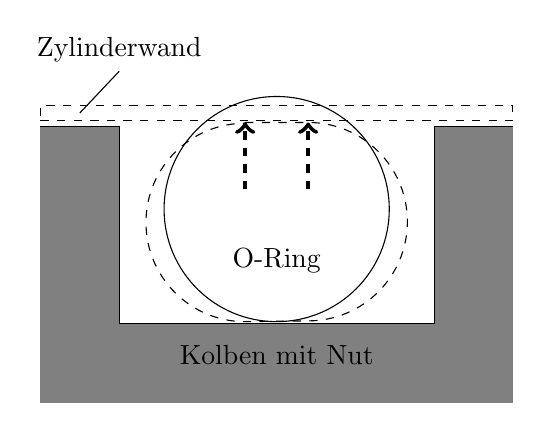
\begin{tikzpicture}
            \draw[gray, fill=gray] (1,0) -- (2,0) -- (2,-2.5) -- (6,-2.5) -- (6,0) -- (7,0) -- (7,-3.5) -- (1, -3.5) -- (1,0) ;
            \draw (1,0) -- (2,0) -- (2,-2.5) -- (6,-2.5) -- (6,0) -- (7,0) ;
            \draw (4,-1.05) circle (1.43);
            \draw[dashed] (1,0.07) -- (7,0.07) -- (7,.27) -- (1,.27) -- (1,.07) ;
            \foreach \x in {3.6, 4.4} \draw[ultra thick, ->, dashed] (\x,-.8) -- (\x,0.05);
            \draw[dashed] (3.6,.05) 
            -- (4.4,.05) 
            arc (90:-90:1.26) 
            -- (3.6,-2.48)
            arc (-90:-270:1.26);

            % Beschriftungen

            \draw (1.5,.17) -- (2.0,.7) node[above] {Zylinderwand};
            \node at (4.0,-2.9)  {Kolben mit Nut};
            \node at (4.0,-1.7) {O-Ring};
        \end{tikzpicture}
